\documentclass[12pt,titlepage,a4paper]{report}

% Texte
\usepackage[utf8]{inputenc}
\usepackage[T1]{fontenc}
\usepackage[french]{babel}
\usepackage[babel=true]{csquotes}
\usepackage{lmodern}
\usepackage{color}
\usepackage{minted}
\usemintedstyle{trac}

% Mise en page
\usepackage{url}
\usepackage[top=2.1cm,bottom=2cm,left=1cm,right=1cm]{geometry}
\usepackage{hyperref}
	\hypersetup{
	colorlinks=false,
	pdfborder={0 0 0},
}
\usepackage{multirow}

% Images
\usepackage{float}
\usepackage{wrapfig}
\usepackage{graphicx}
% Pour inclure des pages PDF
\usepackage[final]{pdfpages}

% Couverture
\usepackage{templateINSA}
\initINSA

\title{Application de gestion de recettes}
\author{Antoine \bsc{Augusti}\\ Thibaud \bsc{Dauce}}

\renewcommand\soustitre{Utilisation de BDD NoSQL pour la réalisation d'une application}
\renewcommand\infoBig{PAO NoSQL}
\renewcommand\infoSmall{ASI4 2014-2015}

%% -- Document
\begin{document}
	\titleINSA{15}{images/fond.png}{0}{-50}{200}{\href{http://upload.wikimedia.org/wikipedia/commons/5/59/Wikimedia_Foundation_Servers-8055_14.jpg}{\textcolor{white}{Licence CC - Wikimedia}}}
	\tableofcontents

	\chapter{Utilisation du framework Laravel}
		Comme énoncé dans la première partie, nous avons fait le choix d'utiliser un framework nommé Laravel. Ce framework est assez récent et a pour objectif de faciliter le développement. Son slogan est \enquote{\textit{PHP that doesn't hurt. Code happy and enjoy the fresh air."}}. Depuis l'année 2013 Laravel a connu un succès important et il est depuis peu le framework PHP attirant le plus de recherches comme montré dans la figure \ref{fig:trends-php-frameworks}.

\begin{figure}[H]
	\centering
	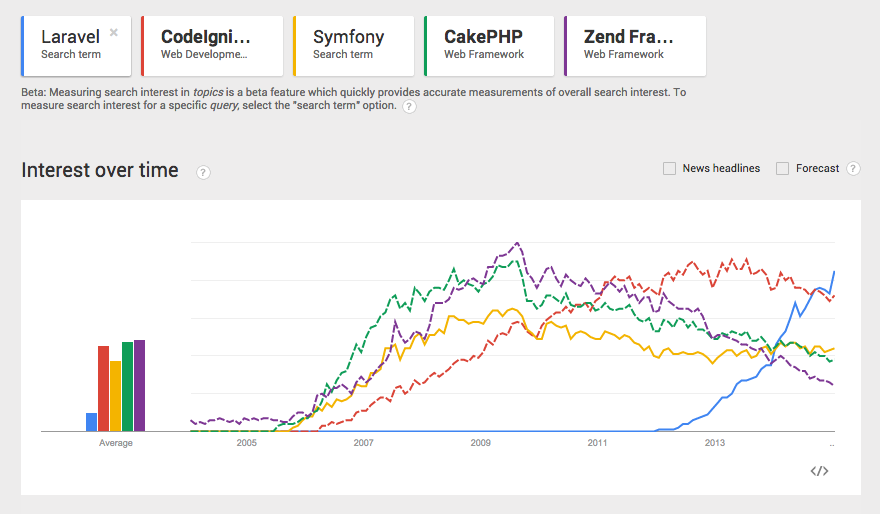
\includegraphics[width=1\textwidth]{images/trends-php-frameworks.png}
	\caption{Recherches Google pour les principaux frameworks PHP.}
	\label{fig:trends-php-frameworks}
\end{figure}

\section{Un framework MVC}
	Laravel est un framework mettant en avant une séparation très importante des modèles, des vues et des contrôleurs. Toutes les classes que nous avons créé se trouvent dans le dossier \verb|app/Insa| et sous l'espace de nom (\textit{namespace}) \verb|Insa|.\\

	Nous avons choisi une architecture modulaire organisée selon les entités. Dans chaque entité, on peut retrouver les dossiers suivants :
	\begin{itemize}
		\item \verb|Controllers| : les contrôleurs associés à l'entité ;
		\item \verb|Models| : les modèles associés à l'entité. Généralement il n'y a qu'une classe dans ce dossier qui correspond au singulier de l'entité, par exemple \verb|\Insa\Recipes\Models\Recipe| ;
		\item \verb|Presenters| : les classes qui ont pour objectif d'effectuer les transformations nécessaires afin de présenter les données brutes dans l'application web ;
		\item \verb|Repositories| : les classes d'accès aux bases de données ;
		\item \verb|Validation| : les classes comportant les règles de validation des entités.
	\end{itemize}

\section{Les \textit{Services Provider}}
	Les \verb|Services Provider| de Laravel sont de simples objets fournissant de la configuration pour l'application. Ils sont définis dans le fichier \verb|app/config/app.php|.\\

	Dans notre cas, nous avons créé un simple Service Provider \verb|LeoCardServiceProvider| qui effectue le lien de l'interface vers l'implémentation dans sa méthode \verb|register|.
	\begin{minted}{php}
	<?php
	public function register()
	{
		$this->app->bind('UserRepository', 'DatabaseUserRepository');
	}
	\end{minted}

\section{L'injection de dépendance}
	Nous n'instançons jamais notre contrôleur, Laravel s'en charge à notre place lorsque la route enregistrée est demandée. Pour instancier une classe, Laravel utilise un outil très puissant de résolution de dépendance grâce à l'introspection de PHP. Avant de créer l'objet nécessaire, elle détermine les classes requises par le constructeur.\\

	Si le constructeur nécessite un objet \verb|DatabaseUserRepository| comme dans notre cas, Laravel va l'instancier et le fournir au constructeur du contrôleur \verb|UsersController|.
	\begin{minted}{php}
	<?php
	public function __construct(DatabaseUserRepository $userRepository)
	{
	$this->userRepository = $userRepository;
	}
	\end{minted}

	De cette manière, nous avons accès au répertoire dans notre contrôleur sans effort.

\section{"Code to an interface"}
	La méthode présentée dans le paragraphe précédent présente l'avantage d'être simple à implémenter mais présente aussi un gros défaut : notre contrôleur est toujours lié à l'ORM via l'objet \verb|DatabaseUserRepository|.\\

	En réalité, notre contrôleur n'a pas besoin de savoir quel type de répertoire il utilise, l'unique besoin est une fonction appelée \verb|getBySerialBatch| prenant en paramètre un tableau d'identifiants NFC et retournant une collection d'utilisateurs. Ce qui est décrit ici est le principe même d'une interface. Nous avons donc créé une interface appelée \verb|UserRepository| et fournissant la signature de méthode requise. Bien évidement, notre répertoire \verb|DatabaseUserRepository| doit maintenant implémenter cette interface.\\

	Nous pouvons donc changer le pré-requis du constructeur de notre contrôleur par l'interface \verb|UserRepository|.
	\begin{minted}{php}
	<?php
	public function __construct(UserRepository $userRepository)
	{
	$this->userRepository = $userRepository;
	}
	\end{minted}

	Mais que va donc faire Laravel lorsqu'il va rencontrer l'interface. En effet, si le framework cherche à résoudre la dépendance, il va se heurter au problème qu'il est impossible d'instancier une interface. Nous avons donc besoin de définir un lien entre notre interface et notre implémentation.

\section{Utilisation d'un répertoire}

	\subsection{Pourquoi utiliser un répertoire}
		Dans le cas d'une application simple comme la notre, il aurait été parfaitement correct d'appeler les méthodes de l'ORM directement dans le contrôleur comme simplifié ci-dessous :
		\begin{minted}{php}
		<?php
		public function batch()
		{
		return User::whereIn('serial', Input::get('data'));
		}
		\end{minted}

		Mais dans le cas d'une application plus complexe, il est préférable de dissocier ses contrôleurs de l'ORM afin d'améliorer la maintenabilité de l'application et de permettre l'utilisation d'un autre système de stockage.

	\subsection{Utilisation d'un répertoire dans notre projet}
		Afin de montrer les possibilités du framework Laravel ainsi que de permettre aux futurs étudiants allant travailler sur l'application de partir sur de bonnes bases, nous avons décidé d'implémenter un répertoire pour les utilisateurs.\\

		Ce répertoire se présente sous la forme d'une classe nommée \verb|DatabaseUserRepository| proposant une seule méthode : \verb|getBySerialBatch|. Cette méthode prend en paramètre un tableau contenant les différents numéros de carte NFC et retourne une collection d'objets \verb|User| via la méthode \verb|whereIn| de l'ORM Eloquent.\\

		Maintenant, afin de découpler nos contrôleurs de l'ORM, nous devons utiliser notre répertoire. Pour cela, Laravel nous propose deux solutions :
		\begin{itemize}
			\item Instancier l'objet normalement dans la méthode ;
			\item Utiliser l'outil d'injection de dépendance de Laravel.
		\end{itemize}

\section{Routes}
	Dans la partie précédente, nous avons les différentes routes nécessaire à la mise en place d'un CRUD. Laravel implémente cela facilement via une façade nommée tout simplement \verb|Route|.

	\begin{minted}{php}
	<?php
	Route::get('users/batch', 'UsersController@batch');
	\end{minted}
	Notre application contient une seule route dans le fichier \verb|app/route.php|, définie comme ci-dessus.\\

	Tout d'abord, nous appelons la méthode \verb|get| parce que dans une optique CRUD, nous cherchons à obtenir des informations. Cette méthode prend en premier paramètre l'URI associé à la route et en deuxième paramètre une chaîne de caractère  formatée comme \verb|ControllerObject@method|. Dans notre cas, lorsque l'utilisateur fait une requête GET sur l'URI \verb|users/batch|, Laravel va appeler la méthode \verb|batch| sur l'objet \verb|UsersController|.

	\subsection{Qu'est-ce qu'une façade}
		Une façade est un classe spécifique qui permet d'appeler des méthodes publiques d'une instance d'un objet via des appels statiques sur la façade.\\

		Par exemple, lorsque j'appelle une méthode statique sur la façade \verb|Route|, Laravel va en réalité appeler une méthode publique d'une instance d'une classe appelée \verb|Illuminate\Routing\Router| stockée dans l'application.\\

		Vous pouvez en savoir plus sur les façades Laravel dans la documentation \url{http://laravel.com/docs/facades}

\section{Le modèle}
	Laravel utilise son propre ORM appelé Eloquent. Ce dernier nécessite la création d'une classe par ressource de l'application. Notre application a donc un modèle nommé \verb|User| situé dans le répertoire \verb|app/models|. Ce dernier hérite du modèle Eloquent qui fournit toutes les méthodes d'accès à la base de données telles que \verb|where|, \verb|find|, \verb|save|...\\

	Dans notre modèle, nous devons définir plusieurs attributs :
	\begin{itemize}
		\item \verb|$table| : cet attribut permet de définir la table associée au modèle. Même si Eloquent est assez intelligent pour définir le pluriel du nom de l'objet (User => users), pour des raisons de lisibilité, nous l'avons redéfini.
		\item \verb|$fillable| : afin de répondre au problème de \verb|MassAssigment|, Eloquent demande de fournir un tableau contenant les attributs du modèle qu'il sera possible de sauvegarder directement via la méthode \verb|create| afin d'éviter qu'un utilisateur mal intentionné insère dans la base de données des champs non voulus. (plus d'informations sur \url{http://laravel.com/docs/eloquent#mass-assignment})
	\end{itemize}

\section{Les contrôleurs}
	Toujours dans une optique CRUD, Laravel nous encourage à créer un contrôleur pour chaque ressource. Notre application ne contient qu'une seule ressource pour le moment appelée \verb|User|, notre contrôleur (par convention) aura donc le nom de \verb|UsersController| et sera situé dans le répertoire \verb|app/controllers|.\\

	Cet objet aura une seule méthode, la méthode \verb|batch| définie dans les routes comme la méthode à appeler.

\section{Conclusion}
	Cette approche par répertoire et par interface nous a permis de créer une application très solide et sans grande dépendance. Par exemple, si nous souhaitons changer d'implémentation, remplacer par exemple la base de données par un système de fichier, il suffit de définir un nouveau répertoire \verb|FileUserRepository| implémentant l'interface \verb|UserRepository| et de compléter les méthodes nécessaires. Ensuite, en changeant le lien dans le Service Provider nous obtenons une nouvelle implémentation sans jamais avoir à ouvrir nos contrôleurs ce qui aurait pu être une source de bugs lors du changement.\\

	La principale limitation de ce système provient du langage PHP, qui ne permet pas de spécifier des types de retour. La nouvelle implémentation doit donc se référer à la documentation et suivre à la lettre les instructions de retour spécifiées dans l'interface même si ces dernières ne sont pas obligatoire au niveau du langage. Ce problème peut être contourné via l'utilisation de la machine virtuelle \verb|HHVM| de Facebook et du langage \verb|Hack|, compatible avec PHP et introduisant un typage statique.

	\section{Conclusion}

	%% Bonnes pratiques
	\subsection{Bonnes pratiques}
		\begin{frame}
			\frametitle{Les bonnes pratiques du NoSQL}

			\begin{itemize}
				\item Ne pas commencer par du NoSQL ;
				\item Bien connaître ses données ;
				\item Ne pas avoir peur de la redondance ;
				\item Ne pas trop redonder ;
				\item Et surtout, bien quantifier ses besoins.
			\end{itemize}


			\begin{block}{RTFM}
				La majorité des bases de données NoSQL connues sur le marché possèdent une très bonne documentation, souvent faite à destination de personnes venant du monde du relationnel.
			\end{block}
		\end{frame}

		\begin{frame}
			\frametitle{D'autres cas d'usage du NoSQL}
			\begin{alertblock}{Première ligne en prod', mais pas que}
				Le NoSQL ne permet pas uniquement de contenir la charge, de répondre aux problématiques du distribué.
			\end{alertblock}

			\vspace{10px}

			D'autres attraits du NoSQL:
			\begin{itemize}
				\item \textbf{Dénormalisation:} business intelligence, machine learning, data mining (BDD colonnes, documents)\dots
				\item \textbf{Stockage:} entrepôt d’agrégation de données (BDD colonnes, documents)
				\item \textbf{Modélisation:} systèmes de recommandation (BDD graphe)
				\item \dots
			\end{itemize}
		\end{frame}

	%% NoSQL ou relationnel ?
	\subsection{NoSQL ou relationnel ?}
		\begin{frame}
			\frametitle{NoSQL ou relationnel ?}

			\begin{alertblock}{Les deux mon capitaine !}
				Les bases de données NoSQL ont été inventées afin de résoudre des problèmes insolubles par les bases de données relationnelle et non \textbf{pas pour les remplacer}.
			\end{alertblock}

			\vspace{20px}

			\begin{tabular}{|l|l|}
				\hline
				\textbf{NoSQL} & \textbf{Relationnel} \\ \hline\hline
				stockage de masse & stockage fiable \\ \hline
				données diverses & données formatées \\ \hline
				scalabilité horizontale & scalabilité verticale \\ \hline
			\end{tabular}
		\end{frame}

		\begin{frame}
			\frametitle{Choix du type de BD NoSQL}

			\begin{tabular}{|p{0.20\textwidth}|p{0.40\textwidth}|p{0.30\textwidth}|}
				\hline
				& Modélisation & Cas d'utilisation \\\hline
				Clé / valeur
				& Modélisation simple, permettant d'indexer des informations diverses via une clé
				& Mise en cache  \\\hline
				Documents
				& Modélisation souple permettant de stocker des documents au format JSON dans des collections
				& Stockage de masse \\\hline
				Graphes
				& Modélisation optimisée pour les problèmes de graphes
				& Stockage provisoire pour traiter les données \\\hline
			\end{tabular}

			\vspace{10px}

			Non exhaustif: il existe d'autres types de BDD NoSQL !
		\end{frame}

\end{document}